\documentclass[12pt]{report}
\usepackage[utf8]{inputenc}
\usepackage[T1]{fontenc}
\usepackage[english]{babel}
\usepackage{graphicx}
\usepackage{amsmath}
\usepackage{amssymb}
\usepackage{hyperref}
\usepackage{epsf}
\usepackage{float}
\usepackage{geometry}
\geometry{hmargin=3.5cm, vmargin=2.5cm}
\usepackage[squaren]{SIunits}
\usepackage{listings}
\usepackage{color}
\definecolor{mygreen}{RGB}{70, 180, 90}
\definecolor{mylilas}{RGB}{255, 117, 45}
\definecolor{cadr}{rgb}{0.89, 0.0, 0.13}
\graphicspath{{DWGs/}}
\usepackage{graphicx}
\usepackage{wrapfig}
\usepackage{graphicx}
\usepackage{multicol}
\usepackage{enumitem}
\usepackage{xcolor}
\usepackage{framed}
\definecolor{listinggray}{gray}{0.9}
\definecolor{lbcolor}{rgb}{0.95,0.95,0.95}
\definecolor{shadecolor}{RGB}{139, 231, 3}


\begin{document}

\lstset{
		backgroundcolor=\color{lbcolor},
   		tabsize=4,    
    	language=C++,
        basicstyle=\sffamily,
        upquote=true,
        aboveskip={1.5\baselineskip},
        columns=fixed,
        showstringspaces=false,
        extendedchars=false,
        breaklines=true,
        numbers=left,
        showtabs=false,
        showspaces=false,
        showstringspaces=false,
        identifierstyle=\ttfamily,
        keywordstyle=\color[rgb]{0,0,1},
        commentstyle=\color[rgb]{0.026,0.5,0.095},
        stringstyle=\color{mylilas},
        numberstyle=\color{black},
		emph={for, break, if, while},
		emphstyle={\color{red}\textbf},
}



\begin{titlepage}
    \begin{center}

		\vspace*{5cm}    

        \Huge
        \textbf{Objectif Morse}
        
        \vspace*{0.5cm}

		\Large

		\textbf{
		\text{-}\text{-}\text{-} \,			%O
		$\cdot\cdot$\text{-} \,\,\,\,\,\,	%U
		$\cdot\cdot\cdot\cdot$ \,			%H
		$\cdot\cdot$ \,						%I
		$\cdot\cdot\cdot$ \,				%S
		\text{-} \,							%T
		\text{-}\text{-}\text{-} \,			%O	
		$\cdot\cdot$ \,						%I
		$\cdot$\text{-}$\cdot$ \,			%R
		$\cdot$}							%E
		
		\textbf{
		\text{-}$\cdot\cdot$ \,				%D
		$\cdot\cdot$\text{-} \,				%U
		\text{-}$\cdot$ \,\,\,\,\,\,		%N
		$\cdot$\text{-} \,					%A
		$\cdot$\text{-}$\cdot\cdot$ \, 		%L
		$\cdot$\text{-}$\cdot\cdot$ \, 		%L
		$\cdot$ \,							%E
		$\cdot$\text{-}$\cdot$}				%R
		
		\textbf{
		$\cdot$ \,							%E
		\text{-} \,\,\,\,\,\,				%T
		$\cdot$\text{-}$\cdot$	\,			%R
		$\cdot$ \,							%E
		\text{-} \,							%T
		\text{-}\text{-}\text{-} \,			%O
		$\cdot\cdot$\text{-} \,				%U
		$\cdot$\text{-}$\cdot$}				%R
		

        \vspace{2cm}
        
        \LARGE
        J. Aleksanderek
        
        K. Zdybal

        \vspace{8.5cm}
        
		\Large

 		November, 2016
	\end{center}
\end{titlepage}

\thispagestyle{empty}
\begin{center}
    
\vspace*{4cm}

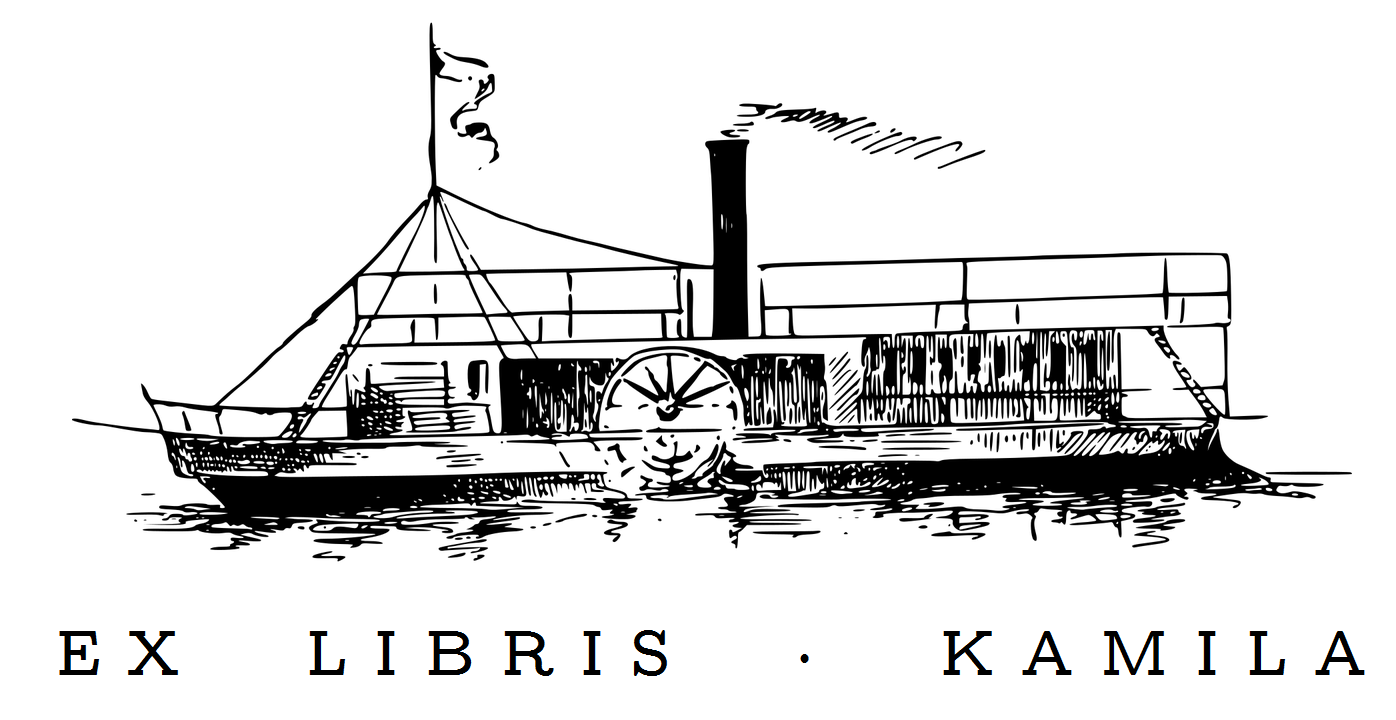
\includegraphics[width = 70mm]{ex_libris.png}

\vspace*{2cm}

Copyright \textcopyright \, Kamila Zdybał, 2016

For more documents similar to this one visit:

https://windengineering.wordpress.com/

or see my other projects on GitHub: @camillejr

To contact me personally drop me a line at:

\verb|kamilazdybal@gmail.com|

\end{center}
\newpage




\setlength{\parindent}{0cm}
\clearpage

\tableofcontents

\setlength{\parskip}{1em}
\renewcommand{\baselinestretch}{1.0}

\chapter{Introduction}\label{chap:intro}

\textbf{Welcome to the Objectif Morse project.} You will soon begin a journey through secret coded messages transmitted between powerful computers over tiny distances. 

The main purpose of this document is to serve as a tutorial for you, if you ever feel like embarking on the same adventure as we did. Following it, you will be able to (hopefully) accomplish the same mission. 

This journey will increase your knowledge in: C++, Linux, Arduino, electronics and, undoubtedly, French language.

It's time to present the mission objectives...

\section{Voici l'Objectif Morse}

You type a secret message on a stationary computer into the terminal. This message is translated into Morse alphabet and the signal of dots and dashes is sent to the parallel port as high and low states. The parallel port's pins are connected to the small circuit with an LED diode, which blinks accordingly to the message translation. Be sure that no spies are observing the diode. This message is received by the phototransistor, situated in the close proximity of an LED. The phototransistor pass on the signal to the Arduino Morse Interpreting Device (AMID\footnote{hint, hint}). Arduino connected to a portable computer prints a translated message in the Arduino console. Be sure that no spies are observing the console. The message is received and the war is won.

\newpage

\subsection{Project phases}

This project is divided into two phases: \textbf{broadcasting} and \textbf{receiving}. The two phases are separated by a 1mm air gap. What really happens inside of the air gap shall forever remain a secret.

\subsection{Motivation pour le projet}

Dans \textit{Tintin au pays de l'or noir}, Tintin est télégraphiste à bord du Speedol Star. Il utilise un émetteur spécial pour transmettre des messages en Morse.

\section{Equipment used}





\newpage

\chapter{Broadcasting}

\verb|OBJECTIF_MORSE, PHASE: BROADCASTING -| The first phase of the Objectif Morse project is to translate the secret message from the regular text to the Morse code. This part introduces the message input using alphanumeric characters in the terminal, where the corresponding program is running. The message is translated by the program and broadcasted on a LED diode connected to the parallel port output pin.

\section{Code description}

The Objectif Morse project is coded in C++ language. It utilises the most powerful part of C++: object-oriented programming.

The code for broadcasting the coded message consists of 5 files plus a makefile. 

The code is split into operating on the messages (\verb|morse.cpp| and \verb|morse.h|) and into sending output on the parallel port (\verb|sendToPort.cpp| and \verb|sendToPort.h|).

There are two header files, one with the class defintion, the other with a function declaration.

The most important constituents of each file are presented in the graph below.


\begin{figure}[H]
\centering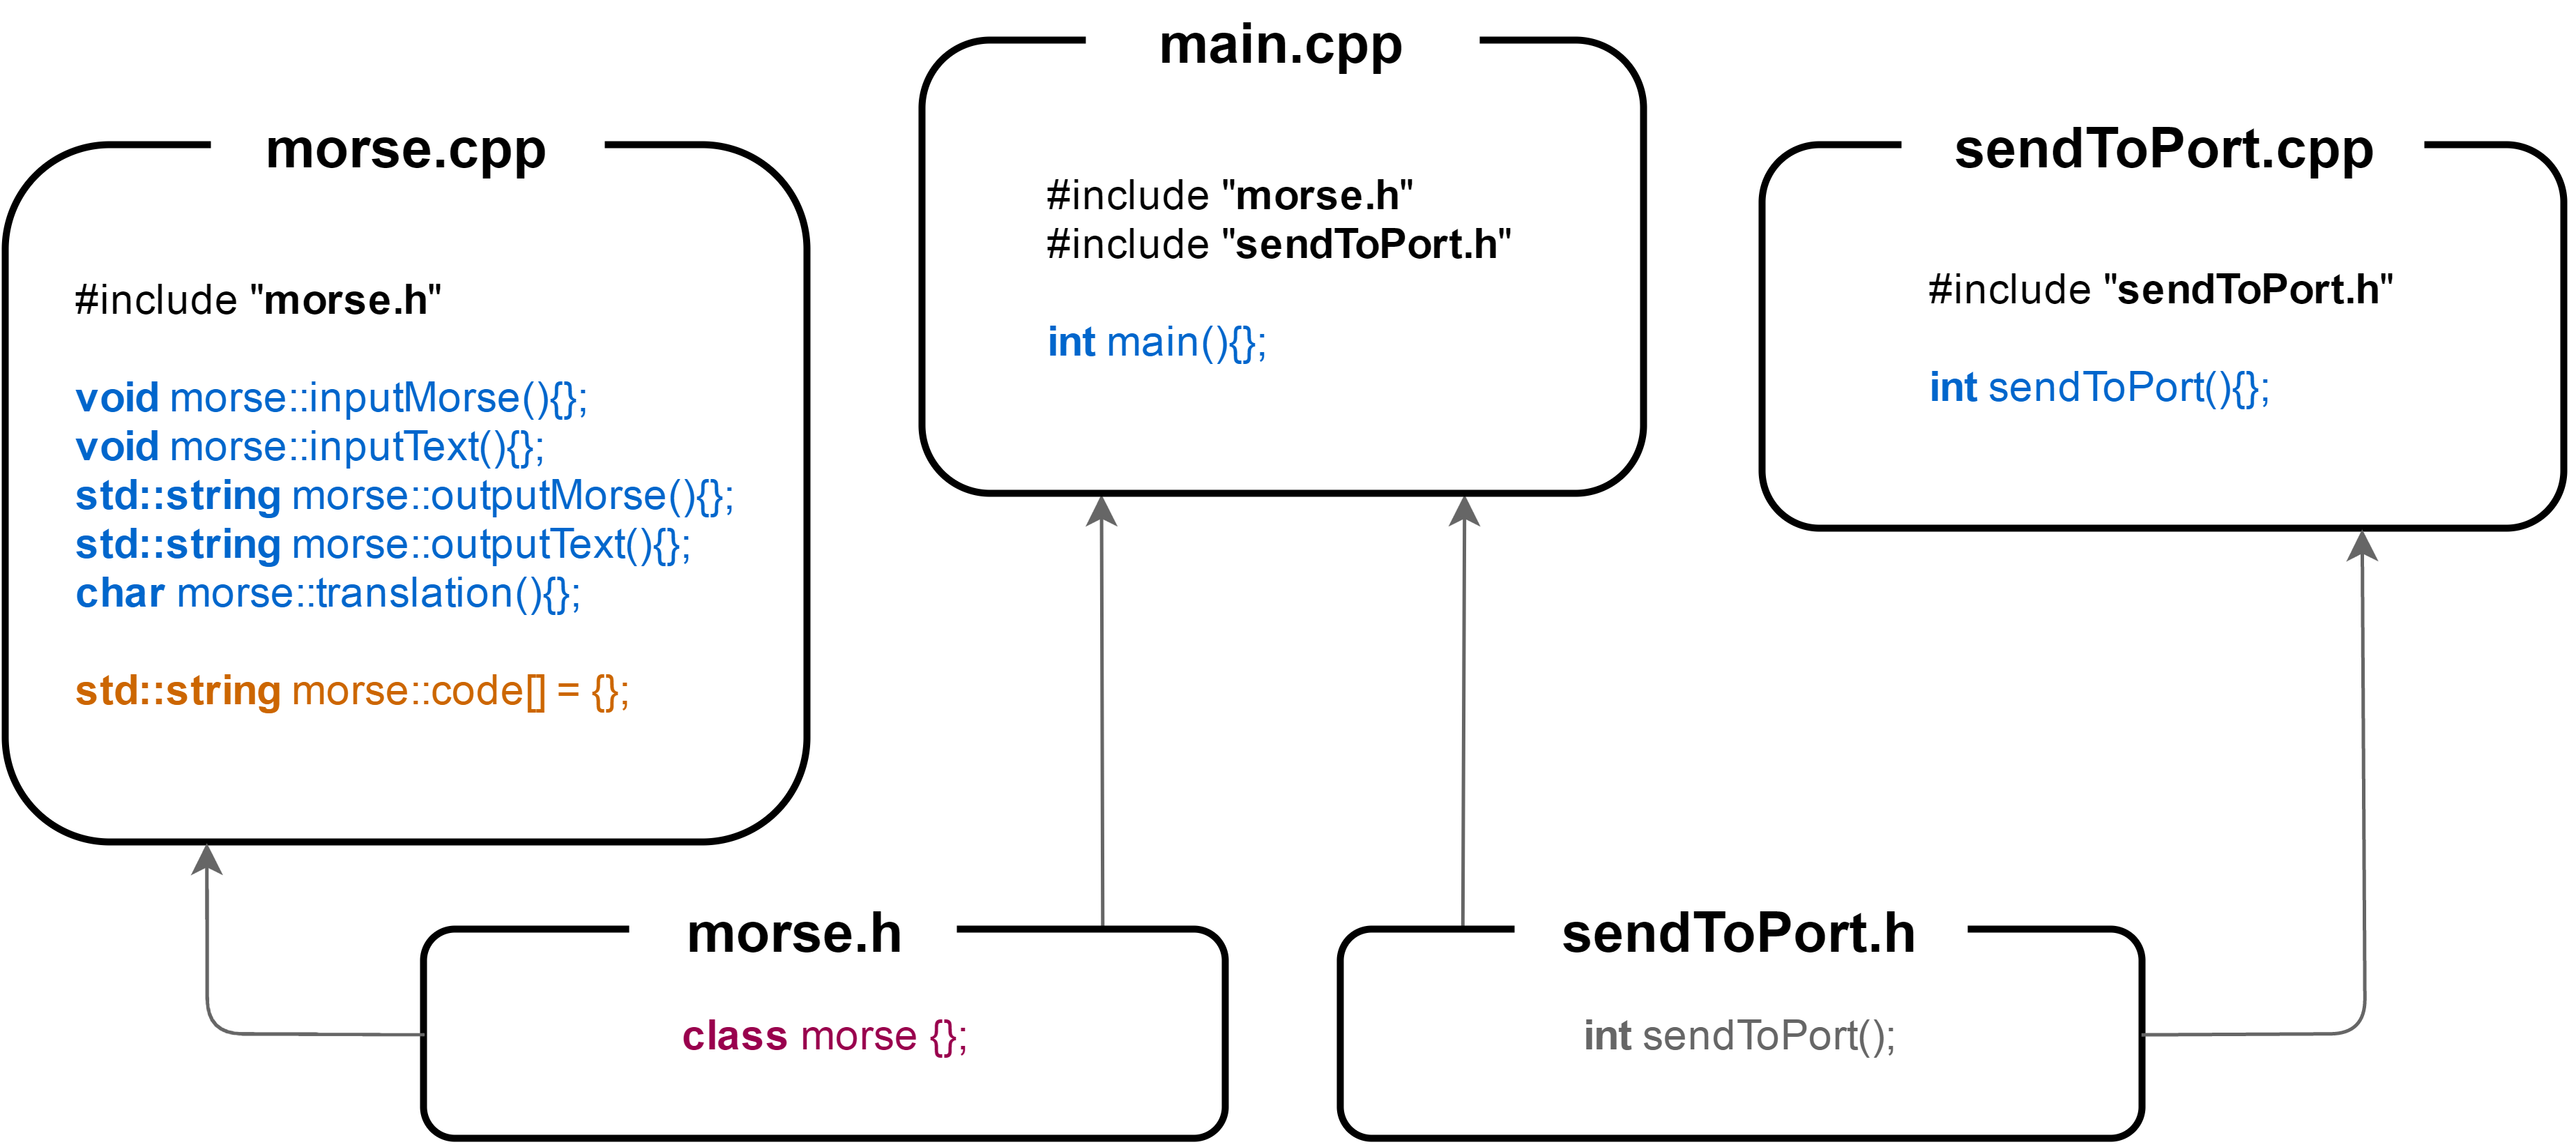
\includegraphics[scale=0.11]{broadcast_code}
\caption{Code structure for \textbf{broadcasting} phase.}				
\label{fig:br_code}
\end{figure}





\subsection{Class morse}

We created a class called \verb|morse| that handles all the necessary variables and functions corresponding to translating from \verb|text > morse| and from \verb|morse > text|.

The definition of the class is presented in the listing below.


\lstinputlisting[label=morse_h, caption=Definition of class \texttt{morse}. File: \texttt{morse.h} ]{morse.h}

We will now describe the class elements, refering to them solely by their name. We start with the class functions:

\verb|inputMorse()| - a public function that takes a string written in Morse alphabet as an input. Ideally, the input string should only consist of the following characters:

\begin{enumerate}
\item dot \verb|"."|

\item dash \verb|"-"|

\item space \verb|" "|

\item slash \verb|"/"|
\end{enumerate}

If the user inputs characters other then the listed above, they will be treated as unknowns in the message.




\verb|inputText()| - a public function that takes a string written in alphanumeric as an input. The input string should only consist of:

\begin{enumerate}
\item letters \verb|A-Z|
\item numbers \verb|0-9|
\item space \verb|" "|
\item dot \verb|"."|
\end{enumerate}

If the user inputs characters other then the listed above, they will be treated as unknowns in the message.


\verb|outputMorse()| - 



\verb|outputText()| - 



\verb|translation()| - 


Following are the class variables:

\verb|morseMessage| - is a private string that contains a message written in the Morse alphabet.


\verb|textMessage| - is a private string that contains a message written in the alphanumeric characters.


\verb|code| - is a private array of strings. A closer description of this array is given in [...]


\subsection{Functions}










\subsection{Sending output to the parallel port}



\subsection{Main}



\subsection{Makefile}



\section{How does it work}



\subsection{Parallel port}



\subsection{Morse code array}



\subsection{ASCII to Morse}


\newpage

\chapter{Receiving}

\verb|OBJECTIF_MORSE, PHASE: RECEIVING -|


\section{Code description}


\section{How does it work}


\chapter{Remarks}

- reading secret alien messages

- laser beam



\begin{snugshade}
\begin{verbatim}
LINUX STUFF
\end{verbatim}
\end{snugshade}


\begin{thebibliography}{50}

\end{thebibliography}

\end{document}
